\documentclass[a5paper, DIV=18, 12pt]{scrartcl}
%\usepackage{balloonspectacular}
\usepackage{multicol}
\setlength\columnsep{0.5cm}
\usepackage{enumitem}
\usepackage[margin=0.925cm]{geometry}


\usepackage{fontspec}
\usepackage[dvipsnames]{xcolor}
\usepackage{tikz}
\setmainfont[Scale=1.0]{Quicksand}
\usepackage{eso-pic}

\setkomafont{section}{\setmainfont[Scale=1.125]{Quicksand-Bold}\LARGE}
\setkomafont{subsection}{\setmainfont{Quicksand-Bold}\Large}
\setkomafont{subsubsection}{\setmainfont{Quicksand-Bold}\large}

% Adjust spacing before and after section headings
\RedeclareSectionCommand[
  runin=false,
  beforeskip=0.75\baselineskip,
  afterskip=0.5\baselineskip
]{section}

% Adjust spacing before and after subsection headings
\RedeclareSectionCommand[
  runin=false,
  beforeskip=0.5\baselineskip,
  afterskip=0.5\baselineskip
]{subsection}

% Adjust spacing before and after subsubsection headings
\RedeclareSectionCommand[
  runin=false,
  beforeskip=0.5\baselineskip,
  afterskip=0.5\baselineskip
]{subsubsection}

\definecolor{eruption_purple}{HTML}{513c3c}
\definecolor{eruption_pink}{HTML}{ff7280}
\definecolor{eruption_orange}{HTML}{fe6737}

\pagestyle{empty}
\raggedright
\begin{document}
\AddToShipoutPictureBG{
\begin{tikzpicture}[remember picture, overlay]
	\node[opacity=0.25] () at (current page.center) {
\includegraphics[width=\pagewidth, height=\pageheight]{Images/newspaper_background2b_a4.jpg}};
\end{tikzpicture}
}

\enlargethispage{1\baselineskip}
\vspace{-1ex}
\begin{center}
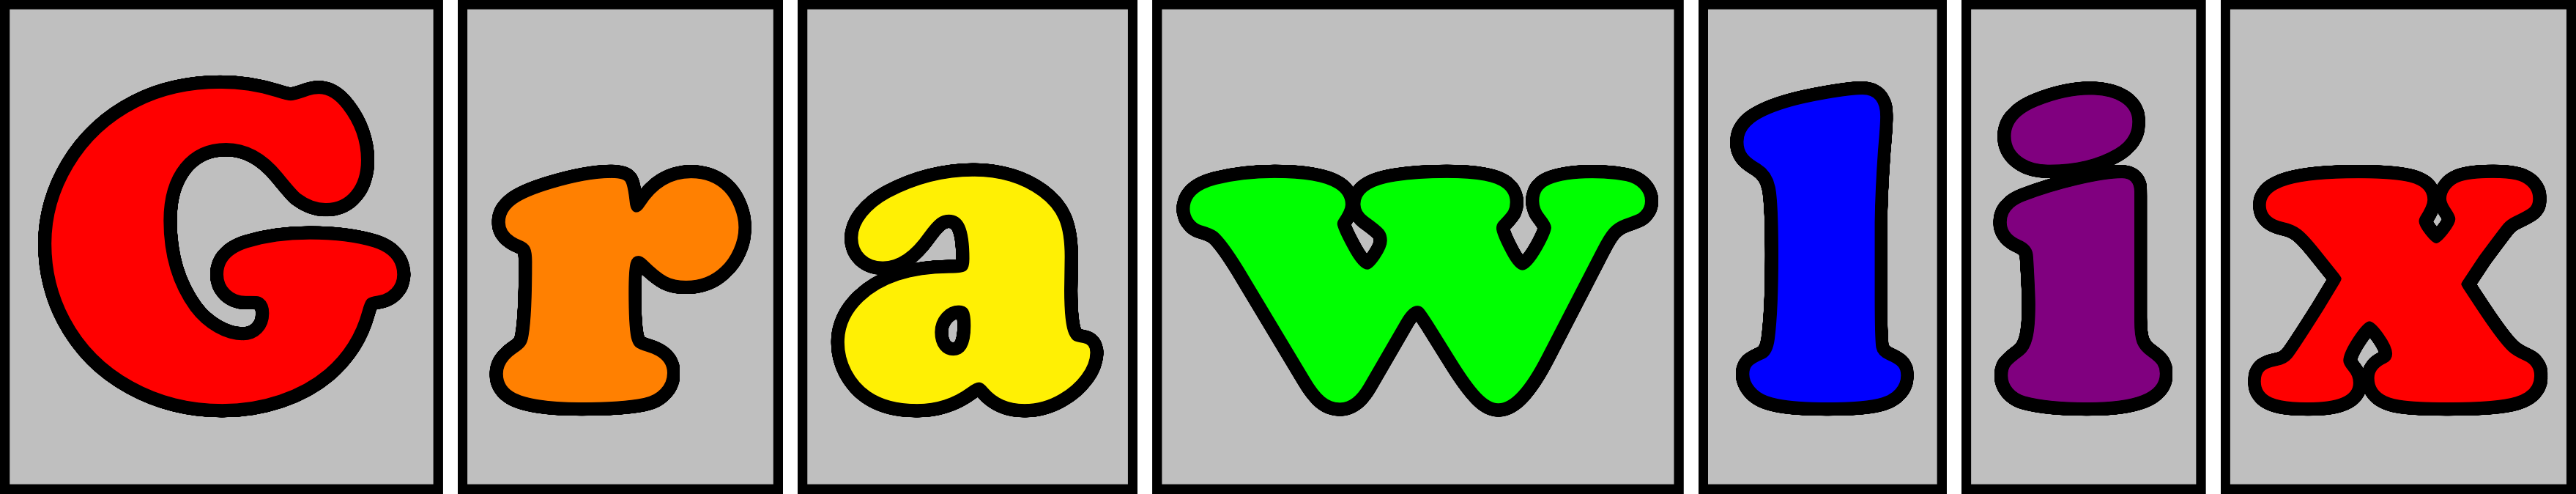
\includegraphics[width=\textwidth]{Images/fancy_title.png}
\setmainfont[Scale=5.455]{Earthquake MF}
\end{center}
\vspace{-0.0ex}

\includegraphics[scale=0.125]{Images/Icons/player_count_icon.png} {\setmainfont[Scale=1.4]{Quicksand-Bold}\Huge \raisebox{6.55pt}{\textcolor{black}{:\ 2}}} \hfill 
\includegraphics[scale=0.125]{Images/Icons/player_age_icon.png} {\setmainfont[Scale=1.4]{Quicksand-Bold}\Huge \raisebox{6.55pt}{\textcolor{black}{:\ 8+}}}\hfill 
\includegraphics[scale=0.125]{Images/Icons/playtime_icon.png} {\setmainfont[Scale=1.4]{Quicksand-Bold}\Huge \raisebox{6.55pt}{\textcolor{black}{:\ 15-30}}}
\vspace{-0.25ex}
\flushleft
\begin{center}{\setmainfont[Scale=1.15]{Quicksand}A strategy game based on the Thirty-Six Officers Problem.}\end{center}% It is suitable for all ages, but is designed for players who are at least eight years old.

\vspace{0.5ex}

\begin{multicols}{2}
\section*{Features}
\begin{itemize}[leftmargin=*, nosep]
\item Extremely simple mechanics that reward skilful play.
\vspace{0.9ex}
\item Mathematically impossible for a game to end in a draw.
\vspace{0.9ex}
\item Tiles that feel great and look amazing on the table.
\vspace{0.9ex}
\item Can be played anywhere with no board required.
\end{itemize}

\section*{Gameplay}
Draft four tiles from the supply.

\vspace{1ex}

On your turn, add a tile from your hand to the grid. Then, refresh your hand.

\vspace{1ex}

Each row and column can have at most one tile of each color and one of each glyph.

\vspace{1ex}

If you cannot add a tile to the grid on your turn, you lose.

\vspace{4ex}

\textbf{Design:} Michael Purcell%

\section*{Components}
Grawlix is played with a set of thirty-six square tiles, one for each combination of six glyphs and six colors.

\vspace{1ex}

\textbf{Note:} If desired, square cards can be used instead of tiles to lower production costs.

\vspace{1.75ex}

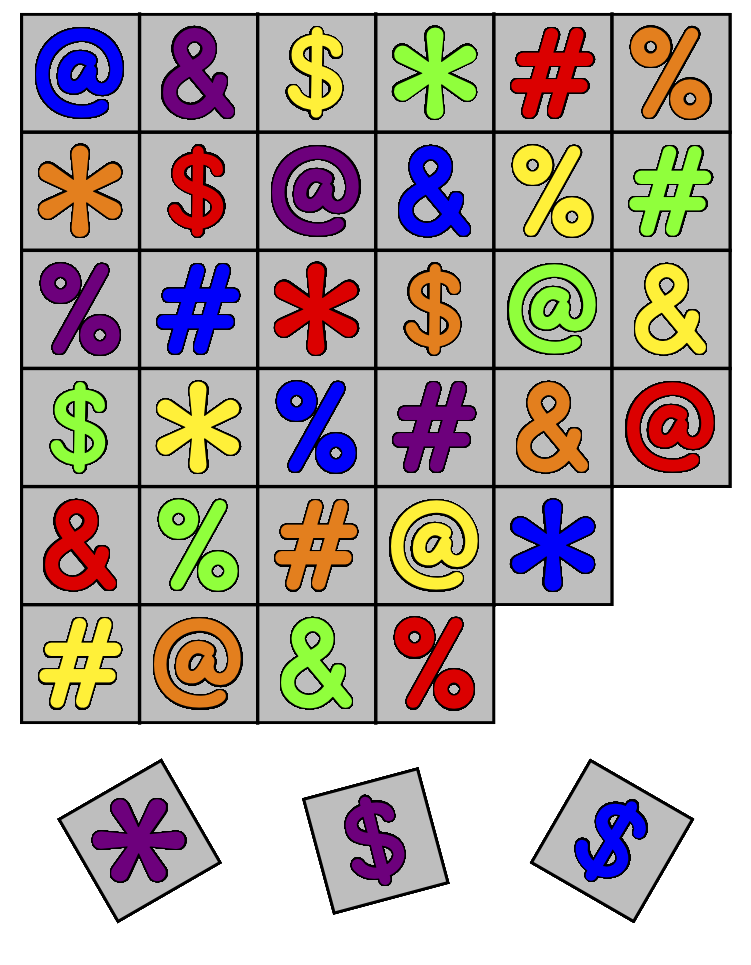
\includegraphics[width=0.95\columnwidth]{Images/cover_image.png}

\vspace{1.75ex}

\textbf{Contact:} mike@armiger.games
\end{multicols}
\end{document}